\chapter{Introduction}


Human-induced climate change is causing dangerous and widespread disruption in nature and affecting the lives of billions of people around the world \cite{ipcc}. 
To tackle climate change and its negative impacts, two main strategies are addressed: climate change adaptation and mitigation. 
Climate change adaptation means finding ways that can help reduce the impacts of climate change on society, the various sectors of its economy, and the places in which we live \cite{handbook}. 
Related projects are in the areas of urban adaptation and land-use planning, resilience of infrastructure, sustainable management of water in drought-prone areas, flood and coastal management, resilience of the agricultural, forestry and tourism sectors, etc. \cite{ec}.  
Climate change mitigating means cutting and sequestering emissions of greenhouse gases (\gls{ghg}) to prevent further increases in their atmospheric concentrations \cite{handbook}. 
Related projects are in the areas of farming, land use, peatland management, renewable energies and energy efficiency; as well as integrated projects that implement climate change mitigation strategies and action plans at regional or national level \cite{ec}. 
%These terms go hand-in-hand as we tackle the climate crisis. 
The newTRENDs project falls into the category of mitigation. 

%Climate change can only be tackled if people actively engage, as consumers and as citizens \cite{clean}. 




%%%%%%%%%%%%%%%%%%%%%%%%%%%%%%%%%%%%%%%%%%%%%%%%%%%
\section{The newTRENDs project}




The historic Paris Agreement sets long-term goals to guide all nations to substantially reduce global \gls{ghg} emissions to limit the global temperature increase to 2 degrees Celsius in this century \cite{paris}. 
To achieve this ambitious goal, the world is facing an unprecedented imperative to a rapidly transition in the energy sector. 
On European Union (\gls{eu}) level, “Energy 2020. A strategy for competitive, sustainable and secure energy”, published in November 2010, and “Energy Roadmap 2050”, published at the end of 2011, are the most important strategy papers currently, pointing the direction for energy developments in the \gls{eu} \cite{roadmap}. 
The aim is to confirm Europe's commitment to lead in global climate action and to present a vision that can lead to achieving net-zero \gls{ghg} emissions by 2050 through a socially-fair transition in a cost-efficient manner \cite{clean}. 

Renewable energy (\gls{re}) and energy efficiency (\gls{ee}) are two central strategies pursued by the \gls{eu} and its Member States concerning the energy system. 
%In 2019, 80.9\% of our total energy supply still depended on burning fossil fuels, namely 26.8\% coal, 30.9\% oil and 23.2\% natural gas \cite{iea}. 
Investments into low-carbon power generation accounted for 15\% recently are expected to rise to more than 30\% by 2030, corresponding to a quadrupling in absolute volumes \cite{shift}. Solar, wind, and the investments for enabling the integration of these technologies to the grid dominate the investments into low-carbon power generation \cite{shift}. 
%Electrification is playing a major role in the energy transition process. 
%Meanwhile, different electrification strategies rely heavily on energy efficiency \cite{electrification}.
Measures to increase energy efficiency, including investments in energy savings and the consolidation of consultancy and information services, are promoted by The National Action Plan on Energy Efficiency (\gls{nape}) \cite{bafa}.  

Transitioning towards a sustainable energy system necessitates significant effort on both the demand and supply sides. 
However, previous research has shown that in many areas energy efficiency gains were counteracted by societal trends that increased corresponding activities, leading to much smaller decreases (or even increases) of energy demand than technologically feasible \cite{2050}. 
The aim of newTRENDs is to increase the qualitative and quantitative understanding of impacts of new societal trends on energy consumption and to improve the modelling of energy demand, energy efficiency and policy instruments \cite{fraunhofer}. 


%%%%%%%%%%%%%%%%%%%%
\subsection{New societal trends on energy demand}


Researchers believe new societal trends have the potential to shift energy demands between sectors and might reinforce or diminish one another when they occur at the same time \cite{2050}. 
%Researchers and organisations are paying increasing attention to how new societal trends are affecting energy demand.
It is therefore important to access current and (foreseeable) future societal trends concerning the impact that they might have on future energy demand \cite{2050}. 

Four arising societal trend clusters that are likely to shape future energy demand in European countries (and worldwide) were established by Brugger et al. \cite{2050}:  
\emph{
  (i) the digitalization of the economy and of private life; 
  (ii) new social and economic models, including the sharing economy and prosumaging (combination of producing, consuming and managing of energy); 
  (iii) industrial transformation, including decarbonization of industrial processes and the circular economy (including a stronger focus on material efficiency); 
  (iv) quality of life, including health effects, urbanization and regionalization. 
}

%\begin{itemize}
%  \item \textbf{Digitalization of life} %\\ the digitalization of the economy and of private life;
%  \item \textbf{New social and economic models} %\\ including the sharing economy and prosumaging (combination of producing, consuming and managing of energy);
%  \item \textbf{Industrial transformation} %\\ including decarbonization of industrial processes and the circular economy (including a stronger focus on material efficiency);
%  \item \textbf{Quality of life} %\\ including health effects, urbanization and regionalization. 
%\end{itemize}

%The newTRENDs project develops the analytical basis for a “2050 Energy Efficiency Vision” by considering new societal trends in energy demand modeling \cite{newtrends}. 
Considering the impact of these new societal trends on energy demand from a closer sectoral perspective,
Yu et al. \cite{newtrends} identified four energy sectors: 

\begin{itemize}
  \item industry, 
  \item transport,  
  \item tertiary, 
  \item residential.  
\end{itemize}

This proposed thesis will focus on residential sector 
while taking scenarios of “consumers” becoming “prosumers” (with \gls{pv}) and “prosumagers” (adding energy storage and \gls{sems}) \cite{consumer} into account.  


%%%%%%%%%%%%%%%%%%%%
\subsection{The modeling of residential buildings}


The FLEX models of the newTRENDs project are referred to as “RC models”,
that calculate (simulate or optimize) the building energy demand at the hourly resolution,
considering the trends of prosumaging households and energy communities, 
which significantly supports the analysis of relevant policies promoting the diffusion of heat pumps (\gls{hp}), \gls{pv}, batteries, and \gls{sems} \cite{newtrends}.


The figure \ref{fig:flex} shows how FLEX interacts with other bottom-up models involved in the newTRENDs project.

\begin{figure}[h]
  \centering
  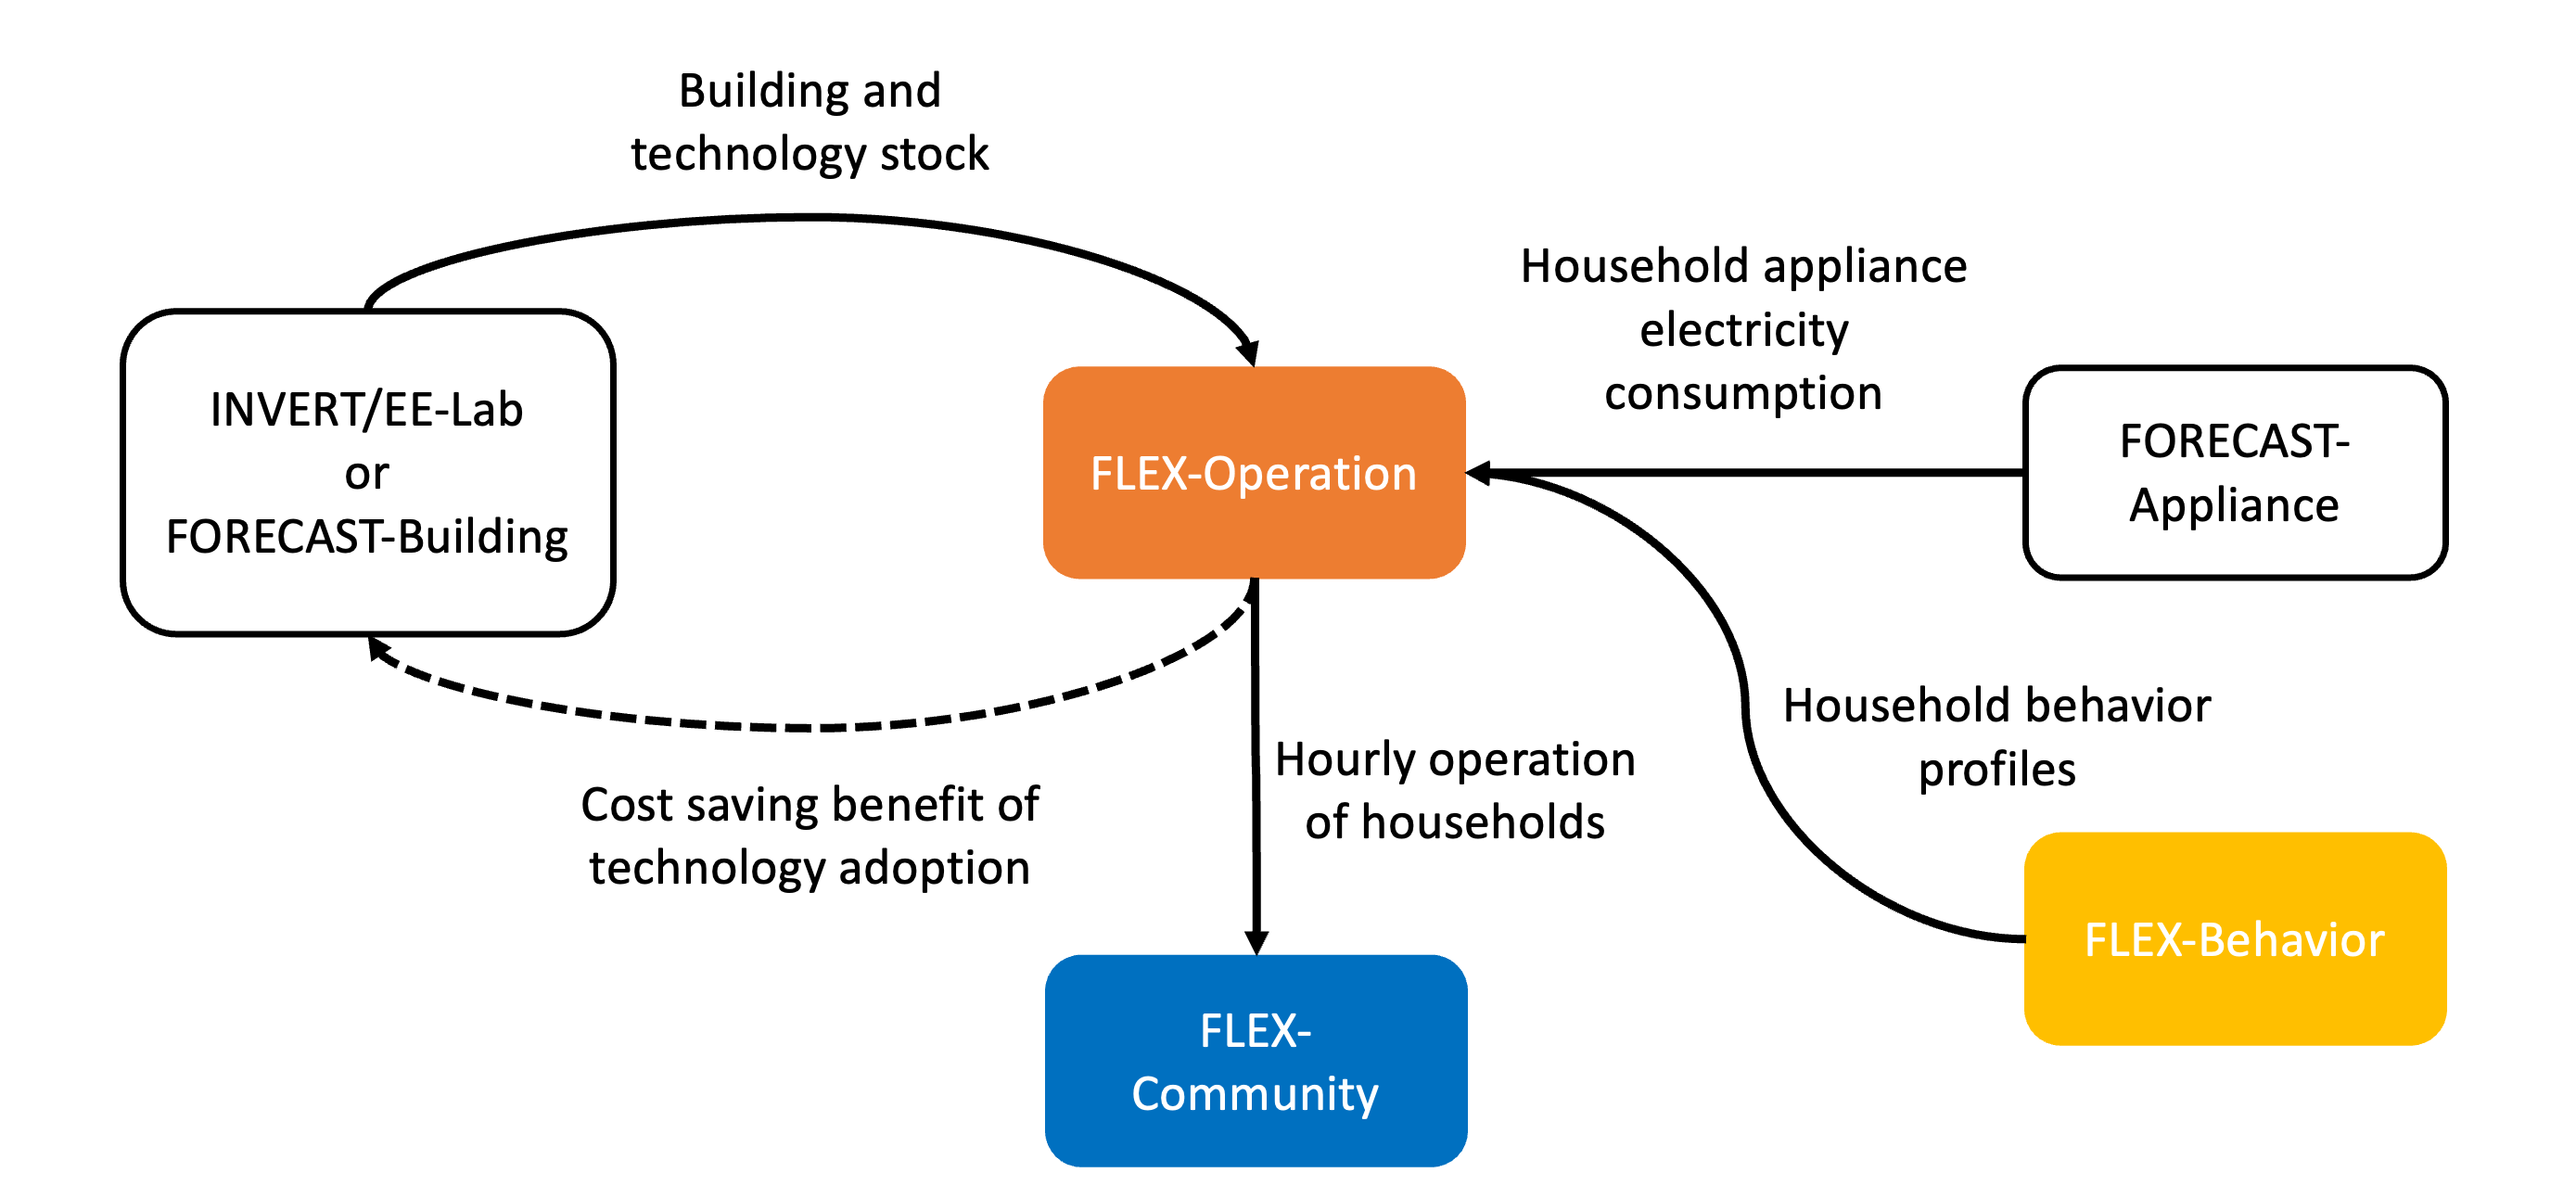
\includegraphics[width=\textwidth]{Images/flex.png}
  \caption{FLEX modeling suite}
  \label{fig:flex}
\end{figure}


%%%%%%%%%%%%%%%%%%%%
\subsubsection{INVERT/EE-Lab and FORECAST-Appliance}


INVERT/EE-Lab and FORECAST-Appliance are the two models that can cover the energy consumption of residential buildings. The two models complement each other and cover the total energy consumption of households. 
However, both INVERT/EE-Lab and FORECAST-Appliance calculate the energy consumption at the annual resolution and cannot model the prosumaging behavior and energy community, which requires an hourly resolution to consider the impact of household behavior, \gls{pv} generation, and energy storage (thermal and battery) on energy consumption. 
In this regard, the FLEX-Operation and FLEX-Community models were developed to improve the building modeling suite and support relevant policy analysis \cite{newtrends}. 


%%%%%%%%%%%%%%%%%%%%
\subsubsection{FLEX-Operation}


FLEX-Operation models the energy system operation of an individual household in hourly resolution.  
It can be used to calculate the energy consumption of each representative building, including operation of technologies (e.g., battery, \gls{pv}, \gls{hp}, etc.) and load profiles in hourly resolution. 
Furthermore, FLEX-Operation can also provide implications for investment decisions, i.e., the energy-saving benefit of technology adoption. 

\begin{figure}[h]
  \centering
  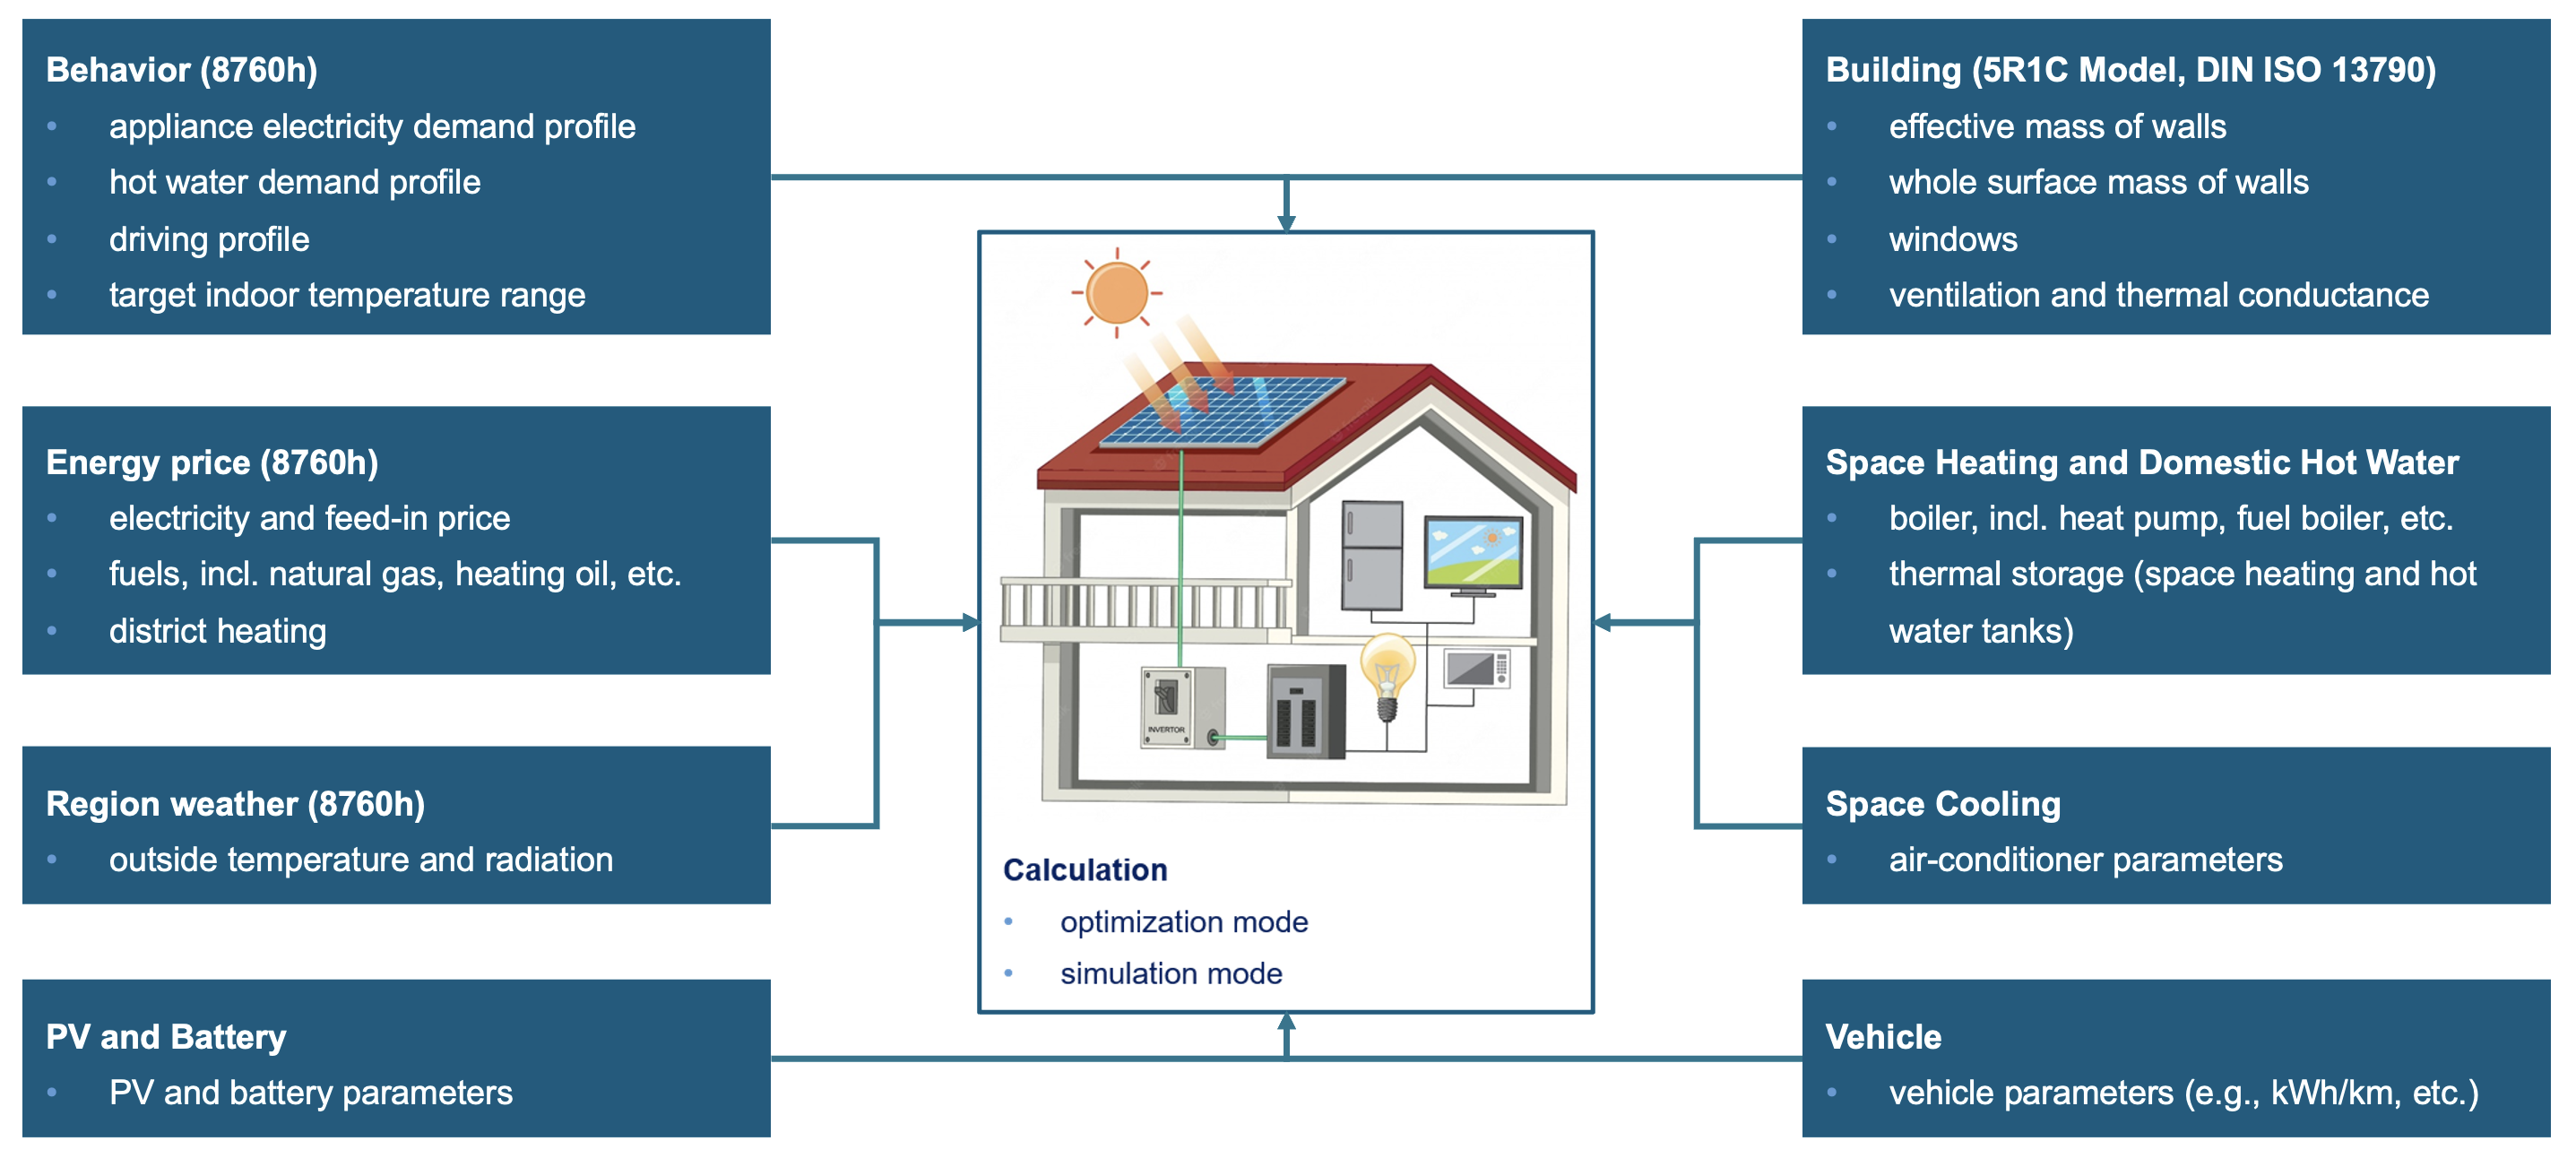
\includegraphics[width=\textwidth]{Images/flex-operation.png}
  \caption{Model structure for individual households}
  \label{fig:flex-operation}
\end{figure}

As shown in figure \ref{fig:flex-operation}, FLEX-Operation considers following five energy services:

\begin{enumerate}
  \item electric appliances, e.g., television, refrigerator, lighting, etc.;
  \item space heating;
  \item domestic hot water;
  \item space cooling;
  \item vehicle. 
\end{enumerate}


%%%%%%%%%%%%%%%%%%%%
\subsubsection{FLEX-Community}


FLEX-Community models the operation of an energy community, i.e., household interaction, aggregator optimisation. 
It can be applied to support the aggregators designing and evaluating business models, as well as making investment decisions, for example, the self-owned battery, \gls{pv} panels, etc.


%%%%%%%%%%%%%%%%%%%%
\subsubsection{FLEX-Behavior}


FLEX-Behavior models the behavior (activity profile) of households' and corresponding load profiles. 
It generates the hourly activity and energy demand profile of a pre-defined individual household. 
The results include: 

\begin{enumerate}
  \item appliance electricity demand,
  \item domestic hot water demand,
  \item driving profile, and
  \item building occupation.
\end{enumerate}




%%%%%%%%%%%%%%%%%%%%%%%%%%%%%%%%%%%%%%%%%%%%%%%%%%%
\section{Motivation and aim}




Buildings will play a central role in the clean energy transition \cite{building}.
High-performance buildings construction and energy renovations reduce the sector’s energy use, digitalisation and smart demand-side management further reduce energy use in buildings \cite{building}.  
As a part of the newTRENDs project, 
the proposed thesis will focus solely on 
the implementation of the FLEX-Operation model.  
The aim is to provide techno-economic assessments 
of configuration optimisations of households' energy systems, 
in order to support decision-making on technology adoption at the residential level. 
Despite the fact that the model primarily responds to societal trends for 2030, 
which means it provides more flexible intergrating technology recommendations when a household already owns a \gls{pv} system, 
this could be, as well, an opportunity to nudge the European households who currently rely on other energy resources
to switch to renewable energy when feasible. 
This project can be used to 
guiding decisions on the use of clean energy and energy technologies at the household level, 
and encouraging households to engage in energy conservation practices and investments. 


%%%%%%%%%%%%%%%%%%%%%%%%%%%%%%%%%%%%%%%%%%%%%%%%%%%
\section{Research gaps and questions}


Regarding the general transition to renewable energy sources, 
there has been a lot of social study and advocacy in the academic community. 
The infrastructure has been transformed with the support of policy makers, 
and the sector is now reaching its maturity. 
It's time to motivate households to actively engage in adjusting their home energy systems.

Empirical results suggest that households' propensity to invest in clean energy technologies depends mainly on home ownership, income, social context and household energy conservation practices,
in addition, environmental attitudes and beliefs, as manifest in energy conservation practices or membership in an environmental non-governmental organisation, also play a relevant role in technology adoption \cite{determinants}.

\colorbox{orange}{Is there any literature review to add?}

This proposed thesis attempts to answer:  
how HCI can help households' investment in energy efficiency and renewables
from a techno-economic perspective.
%evaluations of the technological performance and economic feasibility of a household's energy system.
As well as to develop a user-friendly software for this purpose. 

The following research objectives will aid in achieving the goal: 

\begin{itemize}
  \item Investigating the data required by the FLEX-Operation model. 
  \item Indentifying the typical European household types and understanding their perceptions of the household energy system. 
%  \item Providing recommendations and evaluations of the technological performance and economic feasibility of household's energy system.
  \item Designing the web application with user-centred approaches. 
  \item Using data visualisation techniques to ensure explainability of the recommendations. 
  \item Developing the frontend and backend web application. 
  \item Evaluating the explainability of the recommendations from users' perspectives and measuring the impact of the households perceptions towards proposed solutions. 
  \item Allowing long-term event tracking for design iteration. 
\end{itemize}

%Meanwhile, the following criteria should be taken into consideration 
%while building a software application from a user's perspective: 

%\begin{itemize}
%  \item The software should be easy and effortless to use. 
%  \item The interactions should be intuiative. 
%  \item The assessments should be clear explained to users. 
%\end{itemize}

Accordingly, three subquestions are raised: 

\begin{enumerate}
  \item What are the data required by the FLEX-Operation model from households? 
  \item What are the typical European household profiles? 
  \item How to offer trustworthy and user-friendly recommendations to European households from a techno-economic perspective? 
\end{enumerate}




%%%%%%%%%%%%%%%%%%%%%%%%%%%%%%%%%%%%%%%%%%%%%%%%%%
\section{Supervision and planning} 




The master thesis project is worth 30 Credits at Siegen University. 
This proposed project will discuss both research and application aspects 
related to the crucial topic of techno-economic assessment. 
To meet the design requirements, 
it is expected that scientific review, data analysis, user testing, and evaluating will be involved. 
Thus, the project is believed to be justified for those credits.


\subsection{Supervision}


This master thesis project will be supervised by 
Prof. Dr. Gunnar Stevens (\href{mailto:gunnar.stevens@uni-siegen.de}{gunnar.stevens@uni-siegen.de}) at Siegen University and 
Dr. Songming Yu (\href{mailto:songmin.yu@isi.fraunhofer.de}{songmin.yu@isi.fraunhofer.de}) from The Fraunhofer Institute for Systems and Innovation Research. 


\subsection{Time planning}


The following is the time allocation for the research objetives, 
which are scheduled to be completed in 22 weeks. \\

\begin{table}[h]
    \begin{center}
        \begin{tabular}{ p{0.02\linewidth} p{0.8\linewidth} }
        \hline 
        \cellcolor{yellow!70!lime}1 & Investigating the data required by the FLEX-Operation model to provide recommendations and evaluations of the technological performance and economic feasibility of a household's energy system. \\
        \hline 
        \cellcolor{yellow!60!lime}2 & Indentifying the typical European household types and understanding their perceptions of the household energy system. \\
        \hline 
        \cellcolor{yellow!50!lime}3 & Designing the web application with user-centred approaches. \\
        \hline 
        \cellcolor{yellow!40!lime}4 & Using data visualisation techniques to ensure explainability of the recommendations. \\
        \hline 
        \cellcolor{yellow!30!lime}5 & Developing the frontend and backend web application. \\
        \hline 
        \cellcolor{yellow!20!lime}6 & Evaluating the explainability of the recommendations from users' perspectives and measuring the impact of the households perceptions towards proposed solutions. \\
        \hline
        \cellcolor{yellow!10!lime}7 & Allowing long-term event tracking for design iteration. \\
        \hline 
        \end{tabular}
        \caption{Objectives}
        \label{tab:objectives}
    \end{center}
\end{table}

\renewcommand{\arraystretch}{0.9}
\begin{table}[h]
    \begin{center}
        \begin{tabular}{ r r c c c c c c c }
        && \textbf{1} & \textbf{2} & \textbf{3} & \textbf{4} & \textbf{5} & \textbf{6} & \textbf{7} \\ 
        \multirow{4}{*}{\textbf{Feb}} & w1 & \cellcolor{yellow!70!lime} \\ & w2 & \cellcolor{yellow!70!lime} \\ & w3 && \cellcolor{yellow!60!lime} \\ & w4 && \cellcolor{yellow!60!lime} \\ 
        \multirow{5}{*}{\textbf{Mar}} & w5 && \cellcolor{yellow!60!lime} \\ & w6 &&& \cellcolor{yellow!50!lime} \\ & w7 &&& \cellcolor{yellow!50!lime} \\ & w8 &&& \cellcolor{yellow!50!lime} \\ & w9 &&& \cellcolor{yellow!50!lime} \\ 
        \multirow{4}{*}{\textbf{Apr}} & w10 &&&& \cellcolor{yellow!40!lime} \\ & w11 &&&& \cellcolor{yellow!40!lime} \\ & w12 &&&& \cellcolor{yellow!40!lime} \\ & w13 &&&& \cellcolor{yellow!40!lime} \\ 
        \multirow{4}{*}{\textbf{May}} & w14 &&&&& \cellcolor{yellow!30!lime} \\ & w15 &&&&& \cellcolor{yellow!30!lime} \\ & w16 &&&&& \cellcolor{yellow!30!lime} \\ & w17 &&&&& \cellcolor{yellow!30!lime} \\ 
        \multirow{5}{*}{\textbf{Jun}} & w14 &&&&& \cellcolor{yellow!30!lime} \\ & w15 &&&&& \cellcolor{yellow!30!lime} \\ & w16 &&&&&& \cellcolor{yellow!20!lime} \\ & w17 &&&&&& \cellcolor{yellow!20!lime} \\ & w18 &&&&&& \cellcolor{yellow!20!lime} \\ 
        \multirow{4}{*}{\textbf{Jul}} & w19 &&&&&& \cellcolor{yellow!20!lime} \\ & w20 &&&&&&& \cellcolor{yellow!10!lime} \\ & w21 &&&&&&& \cellcolor{white} \\ & w22 &&&&&&& \cellcolor{white} \\ 
        \end{tabular}
    \end{center}
    \caption{Time planning}
    \label{tab:planning}
\end{table}